% Options for packages loaded elsewhere
\PassOptionsToPackage{unicode}{hyperref}
\PassOptionsToPackage{hyphens}{url}
%
\documentclass[
  11pt,
]{article}
\usepackage{amsmath,amssymb}
\usepackage{iftex}
\ifPDFTeX
  \usepackage[T1]{fontenc}
  \usepackage[utf8]{inputenc}
  \usepackage{textcomp} % provide euro and other symbols
\else % if luatex or xetex
  \usepackage{unicode-math} % this also loads fontspec
  \defaultfontfeatures{Scale=MatchLowercase}
  \defaultfontfeatures[\rmfamily]{Ligatures=TeX,Scale=1}
\fi
\usepackage{lmodern}
\ifPDFTeX\else
  % xetex/luatex font selection
\fi
% Use upquote if available, for straight quotes in verbatim environments
\IfFileExists{upquote.sty}{\usepackage{upquote}}{}
\IfFileExists{microtype.sty}{% use microtype if available
  \usepackage[]{microtype}
  \UseMicrotypeSet[protrusion]{basicmath} % disable protrusion for tt fonts
}{}
\makeatletter
\@ifundefined{KOMAClassName}{% if non-KOMA class
  \IfFileExists{parskip.sty}{%
    \usepackage{parskip}
  }{% else
    \setlength{\parindent}{0pt}
    \setlength{\parskip}{6pt plus 2pt minus 1pt}}
}{% if KOMA class
  \KOMAoptions{parskip=half}}
\makeatother
\usepackage{xcolor}
\usepackage[margin=1in]{geometry}
\usepackage{color}
\usepackage{fancyvrb}
\newcommand{\VerbBar}{|}
\newcommand{\VERB}{\Verb[commandchars=\\\{\}]}
\DefineVerbatimEnvironment{Highlighting}{Verbatim}{commandchars=\\\{\}}
% Add ',fontsize=\small' for more characters per line
\usepackage{framed}
\definecolor{shadecolor}{RGB}{248,248,248}
\newenvironment{Shaded}{\begin{snugshade}}{\end{snugshade}}
\newcommand{\AlertTok}[1]{\textcolor[rgb]{0.94,0.16,0.16}{#1}}
\newcommand{\AnnotationTok}[1]{\textcolor[rgb]{0.56,0.35,0.01}{\textbf{\textit{#1}}}}
\newcommand{\AttributeTok}[1]{\textcolor[rgb]{0.13,0.29,0.53}{#1}}
\newcommand{\BaseNTok}[1]{\textcolor[rgb]{0.00,0.00,0.81}{#1}}
\newcommand{\BuiltInTok}[1]{#1}
\newcommand{\CharTok}[1]{\textcolor[rgb]{0.31,0.60,0.02}{#1}}
\newcommand{\CommentTok}[1]{\textcolor[rgb]{0.56,0.35,0.01}{\textit{#1}}}
\newcommand{\CommentVarTok}[1]{\textcolor[rgb]{0.56,0.35,0.01}{\textbf{\textit{#1}}}}
\newcommand{\ConstantTok}[1]{\textcolor[rgb]{0.56,0.35,0.01}{#1}}
\newcommand{\ControlFlowTok}[1]{\textcolor[rgb]{0.13,0.29,0.53}{\textbf{#1}}}
\newcommand{\DataTypeTok}[1]{\textcolor[rgb]{0.13,0.29,0.53}{#1}}
\newcommand{\DecValTok}[1]{\textcolor[rgb]{0.00,0.00,0.81}{#1}}
\newcommand{\DocumentationTok}[1]{\textcolor[rgb]{0.56,0.35,0.01}{\textbf{\textit{#1}}}}
\newcommand{\ErrorTok}[1]{\textcolor[rgb]{0.64,0.00,0.00}{\textbf{#1}}}
\newcommand{\ExtensionTok}[1]{#1}
\newcommand{\FloatTok}[1]{\textcolor[rgb]{0.00,0.00,0.81}{#1}}
\newcommand{\FunctionTok}[1]{\textcolor[rgb]{0.13,0.29,0.53}{\textbf{#1}}}
\newcommand{\ImportTok}[1]{#1}
\newcommand{\InformationTok}[1]{\textcolor[rgb]{0.56,0.35,0.01}{\textbf{\textit{#1}}}}
\newcommand{\KeywordTok}[1]{\textcolor[rgb]{0.13,0.29,0.53}{\textbf{#1}}}
\newcommand{\NormalTok}[1]{#1}
\newcommand{\OperatorTok}[1]{\textcolor[rgb]{0.81,0.36,0.00}{\textbf{#1}}}
\newcommand{\OtherTok}[1]{\textcolor[rgb]{0.56,0.35,0.01}{#1}}
\newcommand{\PreprocessorTok}[1]{\textcolor[rgb]{0.56,0.35,0.01}{\textit{#1}}}
\newcommand{\RegionMarkerTok}[1]{#1}
\newcommand{\SpecialCharTok}[1]{\textcolor[rgb]{0.81,0.36,0.00}{\textbf{#1}}}
\newcommand{\SpecialStringTok}[1]{\textcolor[rgb]{0.31,0.60,0.02}{#1}}
\newcommand{\StringTok}[1]{\textcolor[rgb]{0.31,0.60,0.02}{#1}}
\newcommand{\VariableTok}[1]{\textcolor[rgb]{0.00,0.00,0.00}{#1}}
\newcommand{\VerbatimStringTok}[1]{\textcolor[rgb]{0.31,0.60,0.02}{#1}}
\newcommand{\WarningTok}[1]{\textcolor[rgb]{0.56,0.35,0.01}{\textbf{\textit{#1}}}}
\usepackage{graphicx}
\makeatletter
\def\maxwidth{\ifdim\Gin@nat@width>\linewidth\linewidth\else\Gin@nat@width\fi}
\def\maxheight{\ifdim\Gin@nat@height>\textheight\textheight\else\Gin@nat@height\fi}
\makeatother
% Scale images if necessary, so that they will not overflow the page
% margins by default, and it is still possible to overwrite the defaults
% using explicit options in \includegraphics[width, height, ...]{}
\setkeys{Gin}{width=\maxwidth,height=\maxheight,keepaspectratio}
% Set default figure placement to htbp
\makeatletter
\def\fps@figure{htbp}
\makeatother
\setlength{\emergencystretch}{3em} % prevent overfull lines
\providecommand{\tightlist}{%
  \setlength{\itemsep}{0pt}\setlength{\parskip}{0pt}}
\setcounter{secnumdepth}{-\maxdimen} % remove section numbering
\ifLuaTeX
  \usepackage{selnolig}  % disable illegal ligatures
\fi
\IfFileExists{bookmark.sty}{\usepackage{bookmark}}{\usepackage{hyperref}}
\IfFileExists{xurl.sty}{\usepackage{xurl}}{} % add URL line breaks if available
\urlstyle{same}
\hypersetup{
  pdftitle={Final Project},
  pdfauthor={Dahye Chung, Donguk Yoo, Hanseung Jang, Sanghyun Lee, Jungyoon Choi, Seokyeong Park, Semin Seo, Boyeon Kim},
  hidelinks,
  pdfcreator={LaTeX via pandoc}}

\title{Final Project}
\author{Dahye Chung, Donguk Yoo, Hanseung Jang, Sanghyun Lee, Jungyoon
Choi, Seokyeong Park, Semin Seo, Boyeon Kim}
\date{2023-07-19}

\begin{document}
\maketitle

\begin{Shaded}
\begin{Highlighting}[]
\FunctionTok{library}\NormalTok{(tidyverse)}
\end{Highlighting}
\end{Shaded}

\begin{verbatim}
## Warning: 패키지 'tidyverse'는 R 버전 4.3.1에서 작성되었습니다
\end{verbatim}

\begin{verbatim}
## Warning: 패키지 'ggplot2'는 R 버전 4.3.1에서 작성되었습니다
\end{verbatim}

\begin{verbatim}
## Warning: 패키지 'tibble'는 R 버전 4.3.1에서 작성되었습니다
\end{verbatim}

\begin{verbatim}
## Warning: 패키지 'tidyr'는 R 버전 4.3.1에서 작성되었습니다
\end{verbatim}

\begin{verbatim}
## Warning: 패키지 'readr'는 R 버전 4.3.1에서 작성되었습니다
\end{verbatim}

\begin{verbatim}
## Warning: 패키지 'purrr'는 R 버전 4.3.1에서 작성되었습니다
\end{verbatim}

\begin{verbatim}
## Warning: 패키지 'dplyr'는 R 버전 4.3.1에서 작성되었습니다
\end{verbatim}

\begin{verbatim}
## Warning: 패키지 'stringr'는 R 버전 4.3.1에서 작성되었습니다
\end{verbatim}

\begin{verbatim}
## Warning: 패키지 'forcats'는 R 버전 4.3.1에서 작성되었습니다
\end{verbatim}

\begin{verbatim}
## Warning: 패키지 'lubridate'는 R 버전 4.3.1에서 작성되었습니다
\end{verbatim}

\begin{verbatim}
## -- Attaching core tidyverse packages ------------------------ tidyverse 2.0.0 --
## v dplyr     1.1.2     v readr     2.1.4
## v forcats   1.0.0     v stringr   1.5.0
## v ggplot2   3.4.2     v tibble    3.2.1
## v lubridate 1.9.2     v tidyr     1.3.0
## v purrr     1.0.1     
## -- Conflicts ------------------------------------------ tidyverse_conflicts() --
## x dplyr::filter() masks stats::filter()
## x dplyr::lag()    masks stats::lag()
## i Use the conflicted package (<http://conflicted.r-lib.org/>) to force all conflicts to become errors
\end{verbatim}

\begin{Shaded}
\begin{Highlighting}[]
\FunctionTok{library}\NormalTok{(broom)}
\end{Highlighting}
\end{Shaded}

\begin{verbatim}
## Warning: 패키지 'broom'는 R 버전 4.3.1에서 작성되었습니다
\end{verbatim}

\begin{Shaded}
\begin{Highlighting}[]
\FunctionTok{library}\NormalTok{(tidyverse)}
\FunctionTok{library}\NormalTok{(tidyr)}
\FunctionTok{library}\NormalTok{(dplyr)}
\end{Highlighting}
\end{Shaded}

\hypertarget{load-the-dataset}{%
\section{Load the dataset}\label{load-the-dataset}}

\begin{Shaded}
\begin{Highlighting}[]
\FunctionTok{library}\NormalTok{(tidyr)}
\FunctionTok{library}\NormalTok{(ggplot2)}
\FunctionTok{library}\NormalTok{(ggmosaic)}
\FunctionTok{library}\NormalTok{(dplyr)}
\NormalTok{Sleep\_health\_and\_lifestyle\_dataset }\OtherTok{\textless{}{-}} \FunctionTok{read\_csv}\NormalTok{(}\StringTok{"Sleep\_health\_and\_lifestyle\_dataset.csv"}\NormalTok{)}
\end{Highlighting}
\end{Shaded}

\begin{verbatim}
## Rows: 374 Columns: 13
## -- Column specification --------------------------------------------------------
## Delimiter: ","
## chr (5): Gender, Occupation, BMI Category, Blood Pressure, Sleep Disorder
## dbl (8): Person ID, Age, Sleep Duration, Quality of Sleep, Physical Activity...
## 
## i Use `spec()` to retrieve the full column specification for this data.
## i Specify the column types or set `show_col_types = FALSE` to quiet this message.
\end{verbatim}

\#\#\#Part 9

\begin{Shaded}
\begin{Highlighting}[]
\FunctionTok{library}\NormalTok{(tidyr)}
\FunctionTok{library}\NormalTok{(ggplot2)}
\FunctionTok{library}\NormalTok{(dplyr)}
\FunctionTok{library}\NormalTok{(readr)}
\FunctionTok{library}\NormalTok{(class)}
\FunctionTok{library}\NormalTok{(caret)}

\NormalTok{Sleep\_health\_and\_lifestyle\_dataset }\OtherTok{\textless{}{-}} \FunctionTok{read\_csv}\NormalTok{(}\AttributeTok{file =} \StringTok{"Sleep\_health\_and\_lifestyle\_dataset.csv"}\NormalTok{,}
  \AttributeTok{col\_types =} \FunctionTok{cols}\NormalTok{(}
    \StringTok{\textquotesingle{}Person ID\textquotesingle{}} \OtherTok{=} \FunctionTok{col\_character}\NormalTok{(),}
    \StringTok{\textquotesingle{}Age\textquotesingle{}} \OtherTok{=} \FunctionTok{col\_double}\NormalTok{(),}
    \StringTok{\textquotesingle{}Sleep Duration\textquotesingle{}} \OtherTok{=} \FunctionTok{col\_double}\NormalTok{(),}
    \StringTok{\textquotesingle{}Stress Level\textquotesingle{}} \OtherTok{=} \FunctionTok{col\_double}\NormalTok{(),}
    \StringTok{\textquotesingle{}Physical Activity Level\textquotesingle{}} \OtherTok{=} \FunctionTok{col\_double}\NormalTok{(),}
    \StringTok{\textquotesingle{}Quality of Sleep\textquotesingle{}} \OtherTok{=} \FunctionTok{col\_double}\NormalTok{(),}
    \StringTok{\textquotesingle{}BMI Category\textquotesingle{}} \OtherTok{=} \FunctionTok{col\_character}\NormalTok{(),}
    \StringTok{\textquotesingle{}Blood Pressure\textquotesingle{}} \OtherTok{=} \FunctionTok{col\_character}\NormalTok{(),}
    \StringTok{\textquotesingle{}Heart Rate\textquotesingle{}} \OtherTok{=} \FunctionTok{col\_double}\NormalTok{(),}
    \StringTok{\textquotesingle{}Daily Steps\textquotesingle{}} \OtherTok{=} \FunctionTok{col\_double}\NormalTok{(),}
    \StringTok{\textquotesingle{}Sleep Disorder\textquotesingle{}} \OtherTok{=} \FunctionTok{col\_character}\NormalTok{()}
\NormalTok{  ))}

\NormalTok{Sleep\_health\_and\_lifestyle\_dataset\_renamed }\OtherTok{\textless{}{-}}\NormalTok{ Sleep\_health\_and\_lifestyle\_dataset }\SpecialCharTok{\%\textgreater{}\%}
  \FunctionTok{rename}\NormalTok{(}\AttributeTok{ID =} \StringTok{\textquotesingle{}Person ID\textquotesingle{}}\NormalTok{,}
         \AttributeTok{Duration =} \StringTok{\textquotesingle{}Sleep Duration\textquotesingle{}}\NormalTok{,}
         \AttributeTok{Stress =} \StringTok{\textquotesingle{}Stress Level\textquotesingle{}}\NormalTok{,}
         \AttributeTok{Physical =} \StringTok{\textquotesingle{}Physical Activity Level\textquotesingle{}}\NormalTok{,}
         \AttributeTok{Quality =} \StringTok{\textquotesingle{}Quality of Sleep\textquotesingle{}}\NormalTok{,}
         \AttributeTok{BMI =} \StringTok{\textquotesingle{}BMI Category\textquotesingle{}}\NormalTok{,}
         \AttributeTok{BPressure =} \StringTok{\textquotesingle{}Blood Pressure\textquotesingle{}}\NormalTok{,}
         \AttributeTok{HRate =} \StringTok{\textquotesingle{}Heart Rate\textquotesingle{}}\NormalTok{,}
         \AttributeTok{DSteps =} \StringTok{\textquotesingle{}Daily Steps\textquotesingle{}}\NormalTok{,}
         \AttributeTok{Disorder =} \StringTok{\textquotesingle{}Sleep Disorder\textquotesingle{}}\NormalTok{)}


\NormalTok{sleep\_data }\OtherTok{\textless{}{-}}\NormalTok{ Sleep\_health\_and\_lifestyle\_dataset\_renamed }\SpecialCharTok{\%\textgreater{}\%}
    \FunctionTok{mutate}\NormalTok{(}\AttributeTok{sufficient\_sleep =}\NormalTok{ Duration }\SpecialCharTok{\textgreater{}=} \FloatTok{7.0}\NormalTok{)}
\end{Highlighting}
\end{Shaded}

\begin{Shaded}
\begin{Highlighting}[]
\NormalTok{sleep\_data }\SpecialCharTok{\%\textgreater{}\%}
  \FunctionTok{pivot\_longer}\NormalTok{(}\AttributeTok{cols =} \FunctionTok{c}\NormalTok{(Disorder), }\AttributeTok{names\_to =} \StringTok{"variable"}\NormalTok{, }\AttributeTok{values\_to =} \StringTok{"value"}\NormalTok{) }\SpecialCharTok{\%\textgreater{}\%}
  \FunctionTok{group\_by}\NormalTok{(variable, value, sufficient\_sleep) }\SpecialCharTok{\%\textgreater{}\%}
  \FunctionTok{summarise}\NormalTok{(}\AttributeTok{count =} \FunctionTok{n}\NormalTok{()) }\SpecialCharTok{\%\textgreater{}\%}
  \FunctionTok{ggplot}\NormalTok{() }\SpecialCharTok{+}
  \FunctionTok{geom\_bar}\NormalTok{(}
    \AttributeTok{mapping =} \FunctionTok{aes}\NormalTok{(}\AttributeTok{x =}\NormalTok{ value, }\AttributeTok{y =}\NormalTok{ count, }\AttributeTok{fill =}\NormalTok{ sufficient\_sleep),}
    \AttributeTok{position =} \StringTok{"dodge"}\NormalTok{,   }
    \AttributeTok{alpha =} \FloatTok{0.6}\NormalTok{,}
    \AttributeTok{stat =} \StringTok{"identity"}
\NormalTok{  ) }\SpecialCharTok{+}
  \FunctionTok{facet\_wrap}\NormalTok{(}\SpecialCharTok{\textasciitilde{}}\NormalTok{ variable, }\AttributeTok{scales =} \StringTok{"free"}\NormalTok{) }\SpecialCharTok{+}
  \FunctionTok{labs}\NormalTok{(}\AttributeTok{x =} \StringTok{"Value"}\NormalTok{, }\AttributeTok{y =} \StringTok{"Count"}\NormalTok{, }\AttributeTok{fill =} \StringTok{"Sufficient Sleep"}\NormalTok{)}
\end{Highlighting}
\end{Shaded}

\begin{verbatim}
## `summarise()` has grouped output by 'variable', 'value'. You can override using
## the `.groups` argument.
\end{verbatim}

\begin{center}\includegraphics[width=0.7\linewidth]{수정_files/figure-latex/unnamed-chunk-4-1} \end{center}

\begin{Shaded}
\begin{Highlighting}[]
\NormalTok{sleep\_data }\SpecialCharTok{\%\textgreater{}\%}
  \FunctionTok{pivot\_longer}\NormalTok{(}\AttributeTok{cols =} \FunctionTok{c}\NormalTok{(Gender), }\AttributeTok{names\_to =} \StringTok{"variable"}\NormalTok{, }\AttributeTok{values\_to =} \StringTok{"value"}\NormalTok{) }\SpecialCharTok{\%\textgreater{}\%}
  \FunctionTok{group\_by}\NormalTok{(variable, value, sufficient\_sleep) }\SpecialCharTok{\%\textgreater{}\%}
  \FunctionTok{summarise}\NormalTok{(}\AttributeTok{count =} \FunctionTok{n}\NormalTok{()) }\SpecialCharTok{\%\textgreater{}\%}
  \FunctionTok{ggplot}\NormalTok{() }\SpecialCharTok{+}
  \FunctionTok{geom\_bar}\NormalTok{(}
    \AttributeTok{mapping =} \FunctionTok{aes}\NormalTok{(}\AttributeTok{x =}\NormalTok{ value, }\AttributeTok{y =}\NormalTok{ count, }\AttributeTok{fill =}\NormalTok{ sufficient\_sleep),}
    \AttributeTok{position =} \StringTok{"dodge"}\NormalTok{,  }
    \AttributeTok{alpha =} \FloatTok{0.6}\NormalTok{,}
    \AttributeTok{stat =} \StringTok{"identity"}
\NormalTok{  ) }\SpecialCharTok{+}
  \FunctionTok{facet\_wrap}\NormalTok{(}\SpecialCharTok{\textasciitilde{}}\NormalTok{ variable, }\AttributeTok{scales =} \StringTok{"free"}\NormalTok{) }\SpecialCharTok{+}
  \FunctionTok{labs}\NormalTok{(}\AttributeTok{x =} \StringTok{"Value"}\NormalTok{, }\AttributeTok{y =} \StringTok{"Count"}\NormalTok{, }\AttributeTok{fill =} \StringTok{"Sufficient Sleep"}\NormalTok{)}
\end{Highlighting}
\end{Shaded}

\begin{verbatim}
## `summarise()` has grouped output by 'variable', 'value'. You can override using
## the `.groups` argument.
\end{verbatim}

\begin{center}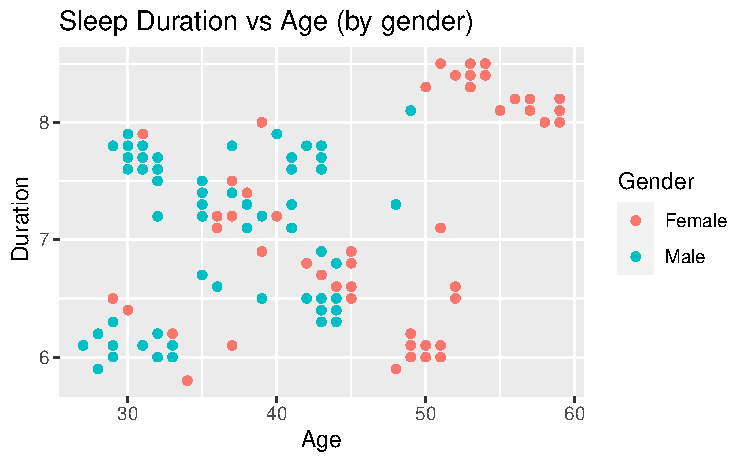
\includegraphics[width=0.7\linewidth]{수정_files/figure-latex/unnamed-chunk-5-1} \end{center}

\begin{Shaded}
\begin{Highlighting}[]
\NormalTok{sleep\_data }\SpecialCharTok{\%\textgreater{}\%}
  \FunctionTok{pivot\_longer}\NormalTok{(}\AttributeTok{cols =} \FunctionTok{c}\NormalTok{(BMI), }\AttributeTok{names\_to =} \StringTok{"variable"}\NormalTok{, }\AttributeTok{values\_to =} \StringTok{"value"}\NormalTok{) }\SpecialCharTok{\%\textgreater{}\%}
  \FunctionTok{mutate}\NormalTok{(}\AttributeTok{value =} \FunctionTok{ifelse}\NormalTok{(value }\SpecialCharTok{==} \StringTok{"Normal"}\NormalTok{, }\StringTok{"Normal Weight"}\NormalTok{, value)) }\SpecialCharTok{\%\textgreater{}\%}
  \FunctionTok{group\_by}\NormalTok{(variable, value, sufficient\_sleep) }\SpecialCharTok{\%\textgreater{}\%}
  \FunctionTok{summarise}\NormalTok{(}\AttributeTok{count =} \FunctionTok{n}\NormalTok{()) }\SpecialCharTok{\%\textgreater{}\%}
  \FunctionTok{ggplot}\NormalTok{() }\SpecialCharTok{+}
  \FunctionTok{geom\_bar}\NormalTok{(}
    \AttributeTok{mapping =} \FunctionTok{aes}\NormalTok{(}\AttributeTok{x =}\NormalTok{ value, }\AttributeTok{y =}\NormalTok{ count, }\AttributeTok{fill =}\NormalTok{ sufficient\_sleep),}
    \AttributeTok{position =} \StringTok{"dodge"}\NormalTok{,   }
    \AttributeTok{alpha =} \FloatTok{0.6}\NormalTok{,}
    \AttributeTok{stat =} \StringTok{"identity"}
\NormalTok{  ) }\SpecialCharTok{+}
  \FunctionTok{facet\_wrap}\NormalTok{(}\SpecialCharTok{\textasciitilde{}}\NormalTok{ variable, }\AttributeTok{scales =} \StringTok{"free"}\NormalTok{) }\SpecialCharTok{+}
  \FunctionTok{labs}\NormalTok{(}\AttributeTok{x =} \StringTok{"Value"}\NormalTok{, }\AttributeTok{y =} \StringTok{"Count"}\NormalTok{, }\AttributeTok{fill =} \StringTok{"Sufficient Sleep"}\NormalTok{)}
\end{Highlighting}
\end{Shaded}

\begin{verbatim}
## `summarise()` has grouped output by 'variable', 'value'. You can override using
## the `.groups` argument.
\end{verbatim}

\begin{center}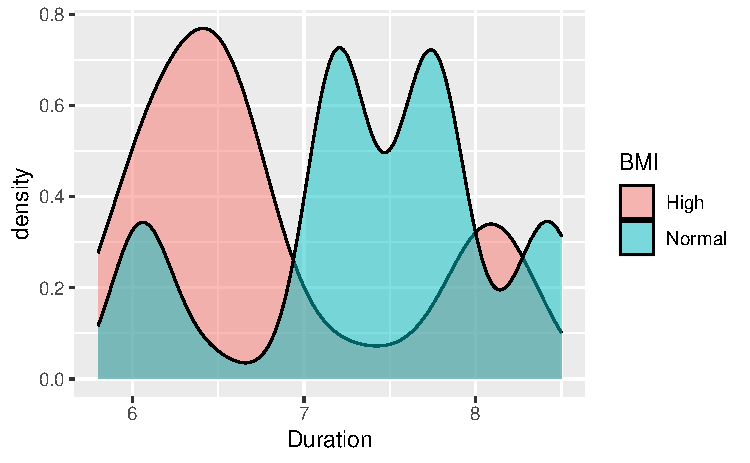
\includegraphics[width=0.7\linewidth]{수정_files/figure-latex/unnamed-chunk-6-1} \end{center}

\begin{Shaded}
\begin{Highlighting}[]
\NormalTok{sleep\_data }\SpecialCharTok{\%\textgreater{}\%}
  \FunctionTok{pivot\_longer}\NormalTok{(}\AttributeTok{cols =} \FunctionTok{c}\NormalTok{(Physical), }\AttributeTok{names\_to =} \StringTok{"variable"}\NormalTok{, }\AttributeTok{values\_to =} \StringTok{"value"}\NormalTok{) }\SpecialCharTok{\%\textgreater{}\%}
  \FunctionTok{group\_by}\NormalTok{(variable, value, sufficient\_sleep) }\SpecialCharTok{\%\textgreater{}\%}
  \FunctionTok{summarise}\NormalTok{(}\AttributeTok{count =} \FunctionTok{n}\NormalTok{()) }\SpecialCharTok{\%\textgreater{}\%}
  \FunctionTok{ggplot}\NormalTok{() }\SpecialCharTok{+}
  \FunctionTok{geom\_bar}\NormalTok{(}
    \AttributeTok{mapping =} \FunctionTok{aes}\NormalTok{(}\AttributeTok{x =}\NormalTok{ value, }\AttributeTok{y =}\NormalTok{ count, }\AttributeTok{fill =}\NormalTok{ sufficient\_sleep),}
    \AttributeTok{position =} \StringTok{"dodge"}\NormalTok{, }
    \AttributeTok{alpha =} \FloatTok{0.6}\NormalTok{,}
    \AttributeTok{stat =} \StringTok{"identity"}
\NormalTok{  ) }\SpecialCharTok{+}
  \FunctionTok{facet\_wrap}\NormalTok{(}\SpecialCharTok{\textasciitilde{}}\NormalTok{ variable, }\AttributeTok{scales =} \StringTok{"free"}\NormalTok{) }\SpecialCharTok{+}
  \FunctionTok{labs}\NormalTok{(}\AttributeTok{x =} \StringTok{"Value"}\NormalTok{, }\AttributeTok{y =} \StringTok{"Count"}\NormalTok{, }\AttributeTok{fill =} \StringTok{"Sufficient Sleep"}\NormalTok{)}
\end{Highlighting}
\end{Shaded}

\begin{verbatim}
## `summarise()` has grouped output by 'variable', 'value'. You can override using
## the `.groups` argument.
\end{verbatim}

\begin{center}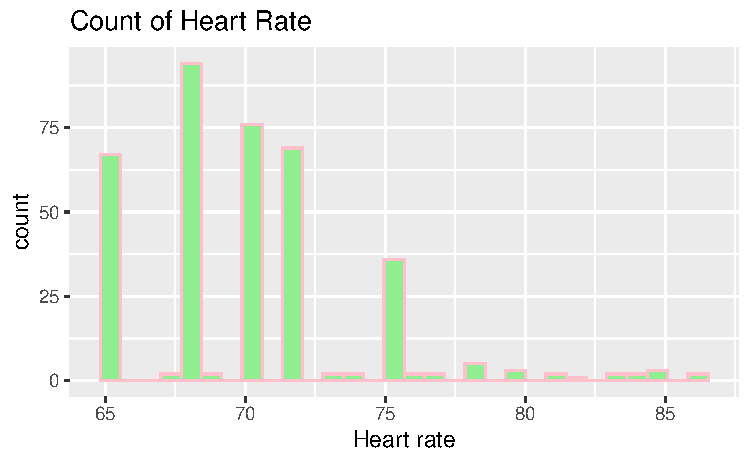
\includegraphics[width=0.7\linewidth]{수정_files/figure-latex/unnamed-chunk-7-1} \end{center}

\begin{Shaded}
\begin{Highlighting}[]
\NormalTok{mode\_gender }\OtherTok{\textless{}{-}} \FunctionTok{as.character}\NormalTok{(}\FunctionTok{names}\NormalTok{(}\FunctionTok{which.max}\NormalTok{(}\FunctionTok{table}\NormalTok{(sleep\_data}\SpecialCharTok{$}\NormalTok{Gender))))}
\NormalTok{mode\_occupation }\OtherTok{\textless{}{-}} \FunctionTok{as.character}\NormalTok{(}\FunctionTok{names}\NormalTok{(}\FunctionTok{which.max}\NormalTok{(}\FunctionTok{table}\NormalTok{(sleep\_data}\SpecialCharTok{$}\NormalTok{Occupation))))}
\NormalTok{mode\_bmi }\OtherTok{\textless{}{-}} \FunctionTok{as.character}\NormalTok{(}\FunctionTok{names}\NormalTok{(}\FunctionTok{which.max}\NormalTok{(}\FunctionTok{table}\NormalTok{(sleep\_data}\SpecialCharTok{$}\NormalTok{BMI))))}

\NormalTok{sleep\_data }\OtherTok{\textless{}{-}}\NormalTok{ sleep\_data }\SpecialCharTok{\%\textgreater{}\%}
\FunctionTok{mutate}\NormalTok{(}
  \AttributeTok{Gender =} \FunctionTok{if\_else}\NormalTok{(}\FunctionTok{is.na}\NormalTok{(Gender), mode\_gender, Gender),}
  \AttributeTok{Occupation =} \FunctionTok{if\_else}\NormalTok{(}\FunctionTok{is.na}\NormalTok{(Occupation), mode\_occupation, Occupation),}
  \AttributeTok{BMI =} \FunctionTok{if\_else}\NormalTok{(}\FunctionTok{is.na}\NormalTok{(BMI), mode\_bmi, BMI)}
\NormalTok{)}
\end{Highlighting}
\end{Shaded}

\begin{Shaded}
\begin{Highlighting}[]
\NormalTok{sleep\_data}\SpecialCharTok{$}\NormalTok{sufficient\_sleep }\OtherTok{\textless{}{-}} \FunctionTok{ifelse}\NormalTok{(sleep\_data}\SpecialCharTok{$}\NormalTok{Duration }\SpecialCharTok{\textgreater{}=} \DecValTok{7}\NormalTok{, }\StringTok{"Sufficient"}\NormalTok{, }\StringTok{"Insufficient"}\NormalTok{)}

\FunctionTok{set.seed}\NormalTok{(}\DecValTok{123}\NormalTok{)}
\NormalTok{train\_indices }\OtherTok{\textless{}{-}} \FunctionTok{createDataPartition}\NormalTok{(sleep\_data}\SpecialCharTok{$}\NormalTok{sufficient\_sleep, }\AttributeTok{p =} \FloatTok{0.7}\NormalTok{, }\AttributeTok{list =} \ConstantTok{FALSE}\NormalTok{)}
\NormalTok{trainingSet }\OtherTok{\textless{}{-}}\NormalTok{ sleep\_data[train\_indices, ]}
\NormalTok{testSet }\OtherTok{\textless{}{-}}\NormalTok{ sleep\_data[}\SpecialCharTok{{-}}\NormalTok{train\_indices, ]}
\end{Highlighting}
\end{Shaded}

\begin{Shaded}
\begin{Highlighting}[]
\NormalTok{trainingSet}\SpecialCharTok{$}\NormalTok{sufficient\_sleep }\OtherTok{\textless{}{-}} \FunctionTok{as.factor}\NormalTok{(trainingSet}\SpecialCharTok{$}\NormalTok{sufficient\_sleep)}
\NormalTok{testSet}\SpecialCharTok{$}\NormalTok{sufficient\_sleep }\OtherTok{\textless{}{-}} \FunctionTok{as.factor}\NormalTok{(testSet}\SpecialCharTok{$}\NormalTok{sufficient\_sleep)}

\NormalTok{training\_Outcomes }\OtherTok{\textless{}{-}}\NormalTok{ trainingSet}\SpecialCharTok{$}\NormalTok{sufficient\_sleep}
\NormalTok{test\_Outcomes }\OtherTok{\textless{}{-}}\NormalTok{ testSet}\SpecialCharTok{$}\NormalTok{sufficient\_sleep}
\end{Highlighting}
\end{Shaded}

\begin{Shaded}
\begin{Highlighting}[]
\NormalTok{model }\OtherTok{\textless{}{-}} \FunctionTok{glm}\NormalTok{(sufficient\_sleep }\SpecialCharTok{\textasciitilde{}}\NormalTok{ Age }\SpecialCharTok{+}\NormalTok{ Gender }\SpecialCharTok{+}\NormalTok{ Occupation }\SpecialCharTok{+}\NormalTok{ Physical }\SpecialCharTok{+}\NormalTok{ DSteps }\SpecialCharTok{+}\NormalTok{ BMI, }\AttributeTok{data =}\NormalTok{ trainingSet, }\AttributeTok{family =}\NormalTok{ binomial)}
\end{Highlighting}
\end{Shaded}

\begin{verbatim}
## Warning: glm.fit: 알고리즘이 수렴하지 않았습니다
\end{verbatim}

\begin{verbatim}
## Warning: glm.fit: 적합된 확률값들이 0 또는 1 입니다
\end{verbatim}

\begin{Shaded}
\begin{Highlighting}[]
\NormalTok{predictions }\OtherTok{\textless{}{-}} \FunctionTok{predict}\NormalTok{(model, }\AttributeTok{newdata =}\NormalTok{ testSet, }\AttributeTok{type =} \StringTok{"response"}\NormalTok{)}

\NormalTok{threshold }\OtherTok{\textless{}{-}} \FloatTok{0.5}  
\NormalTok{predicted\_classes }\OtherTok{\textless{}{-}} \FunctionTok{as.factor}\NormalTok{(}\FunctionTok{ifelse}\NormalTok{(predictions }\SpecialCharTok{\textgreater{}=}\NormalTok{ threshold, }\StringTok{"Sufficient"}\NormalTok{, }\StringTok{"Insufficient"}\NormalTok{))}
\NormalTok{actual\_classes }\OtherTok{\textless{}{-}}\NormalTok{ test\_Outcomes}
\NormalTok{accuracy }\OtherTok{\textless{}{-}} \FunctionTok{sum}\NormalTok{(predicted\_classes }\SpecialCharTok{==}\NormalTok{ actual\_classes) }\SpecialCharTok{/} \FunctionTok{length}\NormalTok{(actual\_classes)}
\FunctionTok{print}\NormalTok{(}\FunctionTok{paste}\NormalTok{(}\StringTok{"Accuracy:"}\NormalTok{, accuracy))}
\end{Highlighting}
\end{Shaded}

\begin{verbatim}
## [1] "Accuracy: 0.981981981981982"
\end{verbatim}

\begin{Shaded}
\begin{Highlighting}[]
\NormalTok{model\_1\_preds }\OtherTok{\textless{}{-}}\NormalTok{ testSet }\SpecialCharTok{\%\textgreater{}\%}
  \FunctionTok{add\_predictions}\NormalTok{(model, }\AttributeTok{type =} \StringTok{"response"}\NormalTok{) }\SpecialCharTok{\%\textgreater{}\%}
  \FunctionTok{mutate}\NormalTok{(}
    \AttributeTok{outcome =} \FunctionTok{as.factor}\NormalTok{(}\FunctionTok{if\_else}\NormalTok{(}\AttributeTok{condition =}\NormalTok{ pred }\SpecialCharTok{\textgreater{}}\NormalTok{ threshold, }
                      \StringTok{"Sufficient"}\NormalTok{, }\StringTok{"Insufficient"}\NormalTok{))}
\NormalTok{  )}
\end{Highlighting}
\end{Shaded}


\end{document}
